\documentclass[runningheads]{llncs}

\usepackage[T1]{fontenc}
\usepackage{graphicx}
\usepackage{amsmath}
\usepackage{amssymb}
\usepackage{url}

\graphicspath{{figures/}}

\begin{document}

\title{Hybrid Modeling}
\titlerunning{Hybrid Modeling}

\author{Manuel Hein}
\authorrunning{M. Hein}

\institute{LMU Munich}

\maketitle

\begin{abstract}
Hybrid modeling combines predictive modeling with generative modeling by
describing the joint distribution as \(p(x,y)=p(y\mid x)p(x)\). This
factorization addresses a weakness of purely discriminative classifiers: a model
for \(p(y\mid x)\) can still assign a confident class prediction to an input that
lies far away from the training distribution. A model for \(p(x)\), in contrast,
can provide information about whether the input itself is plausible. This report
explains the motivation, mathematical background, and main construction of
hybrid models with invertible feature representations. Normalizing flows provide
the key building block because they transform data into latent variables through
bijective maps and allow exact likelihood evaluation through the change of
variables formula. The report follows the derivation from separate generative and
predictive models to shared parameterization, explains the scale mismatch between
classification and density terms, and introduces the weighted hybrid objective.
It then presents Hybrid Integer Discrete Flows as a concrete model for
integer-valued data and discusses the resulting benefits, limitations, and open
questions.

\keywords{Hybrid modeling \and Normalizing flows \and Invertible neural networks
\and Integer discrete flows \and Out-of-distribution detection}
\end{abstract}

\section{Introduction}

Modern machine learning systems often solve decision problems by learning a
conditional distribution \(p(y\mid x)\). In image classification, for example,
\(x\) denotes an image and \(y\) denotes a class label. A discriminative neural
network maps the image to class probabilities and then chooses the most likely
label. This approach has achieved strong empirical performance, but it has a
structural limitation: the conditional distribution does not model whether the
input \(x\) itself is typical of the training data. The model is asked to choose
among known classes even when the input comes from an unfamiliar part of the
input space.

This limitation matters because confidence is not the same as understanding.
A classifier can be far away from its training distribution and still assign a
large probability to one class. From the perspective of the classifier, every
input must pass through the same decision mechanism. If the model has no
component that evaluates \(p(x)\), it cannot directly express that an input is
unusual. Figure~\ref{fig:confidence-flip} illustrates this intuition: a small
change in the input can shift the predicted class probabilities, even though the
input may appear nearly unchanged at the semantic level. The point of the figure
is not that all small perturbations are dangerous, but that a conditional model
alone has no explicit notion of input plausibility.

\begin{figure}
\centering
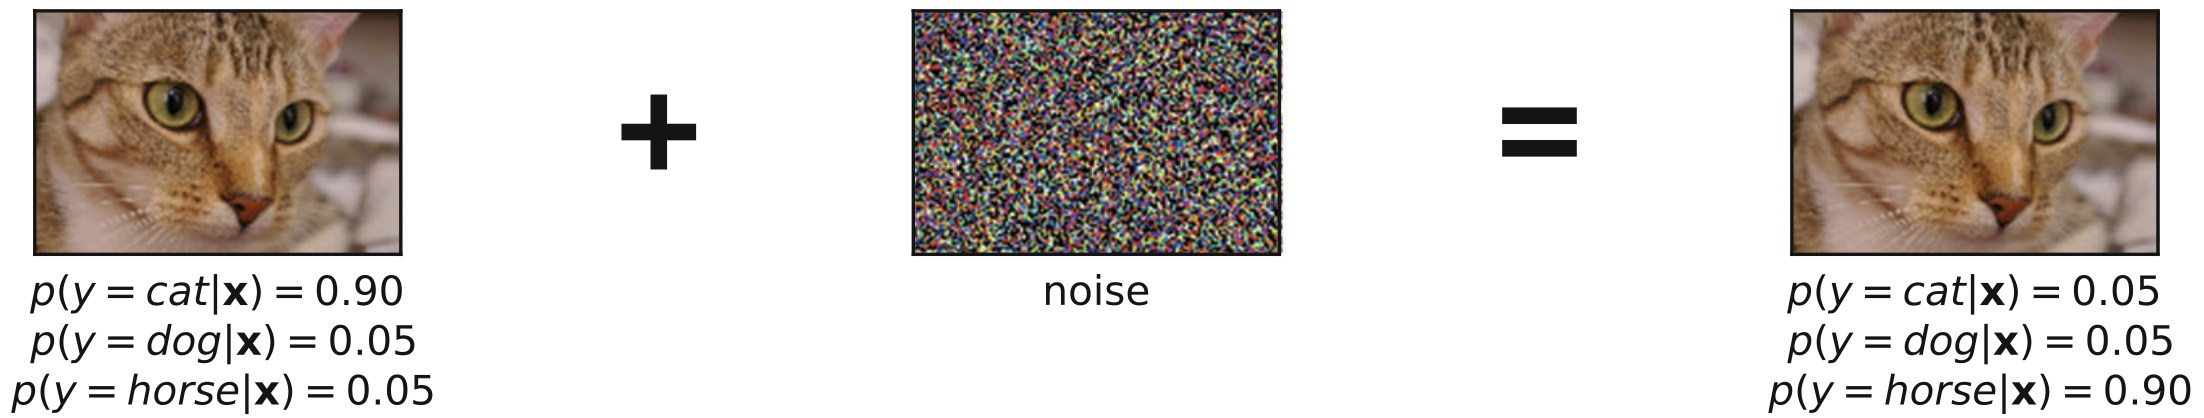
\includegraphics[width=\textwidth]{fig_1_1_confidence_flip.png}
\caption{Conceptual illustration of a confidence failure. A small change in the
input can shift the class probabilities of a purely predictive model, because
the model must still assign probability mass over the available labels. The
figure is an original conceptual redraw inspired by the motivating example in
the book~\cite{tomczak2024deep}.}
\label{fig:confidence-flip}
\end{figure}

Hybrid modeling addresses this problem by modeling the joint distribution of
inputs and labels. The factorization used throughout this report is
\begin{equation}
p(x,y)=p(y\mid x)p(x).
\label{eq:joint-factorization}
\end{equation}
The first factor remains predictive: it answers which label should be assigned
to a given input. The second factor is generative: it answers whether the input
is plausible under the data distribution. Combining both factors gives a richer
description than either factor alone. A model can make a class prediction and
also provide an input plausibility score.

The direction of the factorization matters for the report's emphasis. The model
does not abandon the supervised task; it keeps \(p(y\mid x)\) as the predictive
component and adds \(p(x)\) as a model of the input distribution. Hybrid modeling
is therefore best understood as distribution-aware prediction rather than as
pure generation with labels attached.

Figure~\ref{fig:disc-vs-hybrid} shows the basic contrast. A discriminative
classifier learns a decision boundary. A point far from the observed data can
still be classified confidently if it lies on one side of that boundary. A hybrid
model can use the density \(p(x)\) to notice that the same point is far from the
regions of high probability mass. In that case, the model can treat the decision
as uncertain or at least suspicious. This logic motivates the central question of
the report: how can a single model learn both useful predictive features and a
useful density model?

\begin{figure}
\centering
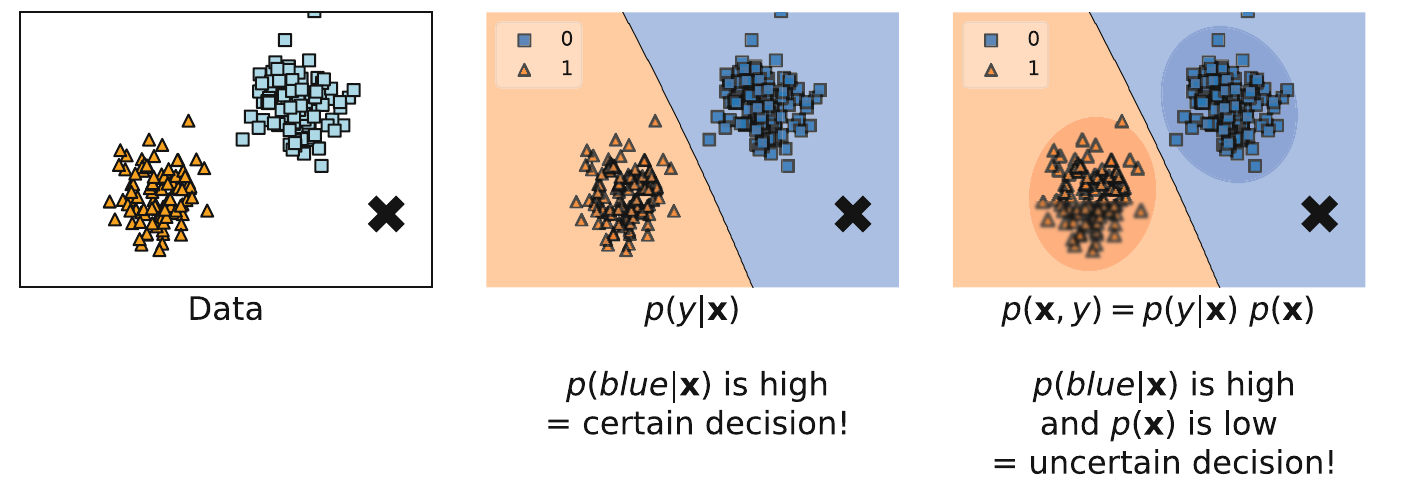
\includegraphics[width=\textwidth]{fig_1_2_discriminative_vs_hybrid.png}
\caption{Conceptual comparison between a purely discriminative classifier and a
hybrid model. A discriminative model assigns a class label based on the decision
boundary even when a new point lies far from the training distribution. A hybrid
model also evaluates \(p(x)\), so the same point can be treated as uncertain or
out-of-distribution. The figure is an original conceptual redraw inspired by the
book's motivation for hybrid modeling~\cite{tomczak2024deep}.}
\label{fig:disc-vs-hybrid}
\end{figure}

The rest of the report follows the development in the book's chapter on hybrid
modeling~\cite{tomczak2024deep}. Section~\ref{sec:background} introduces the
probabilistic and flow-based background. Section~\ref{sec:main} derives the
hybrid objective from the joint factorization, explains why shared
parameterization is useful, and presents the scale mismatch that motivates
weighting. The section then turns to Hybrid Integer Discrete Flows, which adapt
the idea to integer-valued data. Section~\ref{sec:discussion} discusses the
outcomes and open questions suggested by the book's example. The conclusion
summarizes the conceptual contribution of hybrid modeling.

\section{Background}
\label{sec:background}

\subsection{Discriminative, Generative, and Hybrid Models}

The distinction between discriminative and generative modeling is a useful
starting point. A discriminative model learns \(p(y\mid x)\), the distribution
over targets given an input. For classification, this distribution is often
parameterized by a neural network followed by a softmax layer. The model is
optimized to separate labels well, and the geometry of the learned representation
is shaped by predictive performance.

A generative model for the same input instead learns \(p(x)\). This distribution
does not directly answer which class label is correct, but it describes where
data are likely to occur. In the book's framing, this distribution is useful for
more than sampling new objects. It also provides a language for uncertainty about
the environment: an input with low probability under \(p(x)\) may be unfamiliar,
noisy, corrupted, or outside the training distribution~\cite{tomczak2024deep}.

A hybrid model combines these two views through
Eq.~\eqref{eq:joint-factorization}. This factorization is especially appropriate
when the goal is reliable decision-making. The alternative factorization
\(p(x,y)=p(x\mid y)p(y)\) is also valid and is often natural for
class-conditional generation. However, this report follows the book's emphasis:
the goal is not primarily to sample an object from a chosen class, but to support
prediction while retaining information about whether the input itself is
plausible.

\subsection{Normalizing Flows and Change of Variables}

Hybrid models need a tractable model for \(p(x)\). Chapter~4 of the book
introduces normalizing flows as one such model family~\cite{tomczak2024deep}. A
normalizing flow uses an invertible transformation between data and latent
variables. Following the book's notation, the latent variable is written as
\[
z=f^{-1}(x),
\]
where \(f\) maps latent variables back to data and \(f^{-1}\) maps data to
latent variables. The latent distribution \(\pi(z)\) is chosen to be simple, for
example a standard Gaussian distribution. The invertible transformation then
warps this simple distribution into a more flexible distribution over \(x\).

The word ``invertible'' is crucial. In a standard feed-forward classifier, a
feature extractor may intentionally discard information that is irrelevant for
label prediction. Such compression can help classification, but it makes exact
density evaluation difficult because the original input cannot be reconstructed
from the representation. A normalizing flow avoids that loss of information by
requiring a bijective transformation. Each input corresponds to exactly one
latent point, and each latent point corresponds to exactly one input. The model
can therefore use the latent point as a feature representation without giving up
the ability to compute the probability of the original input.

For continuous variables, the likelihood follows from the change of variables
formula:
\begin{equation}
p(x)=\pi\!\left(z=f^{-1}(x)\right)|J_f(x)|^{-1}.
\label{eq:flow-likelihood}
\end{equation}
Here \(J_f\) denotes the Jacobian determinant associated with the transformation
from latent space to data space. More precisely, the determinant is evaluated at
the latent point corresponding to \(x\). The shorthand in
Eq.~\eqref{eq:flow-likelihood} follows the book's notation and emphasizes the
dependency on the observed input. The base-density term measures whether the
latent representation is plausible under \(\pi\). The Jacobian term corrects for
the local volume change induced by the transformation.

The Jacobian determinant is easiest to interpret geometrically. If the mapping
expands a small region of latent space into a larger region of data space, then
probability mass becomes spread out and the density decreases. If the mapping
contracts volume, the density increases. The determinant in
Eq.~\eqref{eq:flow-likelihood} performs exactly this correction. Without the
correction, the model would treat the base density value at \(z=f^{-1}(x)\) as
the data density, ignoring the fact that the transformation may stretch or
compress space. The change of variables formula is therefore what turns an
invertible neural network into a normalized probability density.

Flows become especially useful when \(f\) is built as a composition of
invertible functions. If \(f=f_K\circ\cdots\circ f_1\), then the log-likelihood
can be written as a base log-density minus a sum of log-Jacobian terms:
\begin{equation}
\ln p(x)
=
\ln \mathcal{N}\!\left(z_0=f^{-1}(x)\mid 0,I\right)
-
\sum_{i=1}^{K}\ln |J_{f_i}(z_{i-1})|.
\label{eq:flow-loglikelihood}
\end{equation}
This equation explains the appeal of flow models for hybrid modeling. The same
invertible neural network can produce a useful feature representation \(z\) and
also provide an exact likelihood contribution for \(p(x)\).

The composition view also explains why flow architectures are designed around
tractability. A flexible invertible transformation is useful only if the inverse
map and determinant terms can still be evaluated efficiently. Hybrid modeling
relies on this property when it adds \(\ln p(x)\) to the predictive objective:
the density term must be available during training, not merely in principle.

\subsection{Predictive Heads on Invertible Features}

Once the model has learned an invertible representation, a predictive head can be
placed on top of the latent features. Nalisnick et al. describe this idea as a
model with deep invertible features and a generalized linear model on the feature
space~\cite{nalisnick2019hybrid}. The book's implementation example uses a
small neural classification head instead of emphasizing the generalized linear
model terminology~\cite{tomczak2024deep}. The important shared idea is that the
predictive component and the density component use the same invertible backbone.

This sharing matters for two reasons. First, it avoids training a density model
and a classifier as unrelated systems. Second, it allows the labels to influence
the learned representation while the density objective still preserves
information about the structure of the input space. In this way, the latent
representation can serve two roles: it can be predictive for \(y\), and it can be
probabilistically meaningful for \(x\).

This design creates a useful tension. A purely discriminative representation can
collapse directions that do not affect the label, while a density model cannot
freely discard such directions because it must still explain the input. A hybrid
representation therefore has the potential to be more informative than a
classifier-only representation. At the same time, the two goals need not agree.
Some details of an image may be important for likelihood but irrelevant for the
label; some label-discriminating features may represent small differences in
density. The weighted objective is the mechanism used to manage this tension.

\section{Main Content / Results}
\label{sec:main}

\subsection{Naive Composition and Shared Parameterization}

The hybrid modeling chapter starts from the joint factorization
\begin{equation}
p(x,y)=p(y\mid x)p(x).
\tag{6.1}
\label{eq:book-6-1}
\end{equation}
Equation~\eqref{eq:book-6-1} is the conceptual starting point for the whole
construction. It states that the model should assign high joint probability only
when two conditions hold at the same time: the label is likely given the input,
and the input is likely under the data distribution. A confident class
prediction is not enough if the input itself has low plausibility. Likewise, a
plausible input is not enough if the model assigns low probability to the
correct label. The hybrid score is useful because it keeps these two conditions
visible in the same mathematical object.

A first, naive construction trains the classifier and the density model
separately. If the classifier has parameters \(\alpha\) and the density model has
parameters \(\beta\), the log-joint is
\begin{equation}
\ln p(x,y)
=
\ln p_{\alpha}(y\mid x)+\ln p_{\beta}(x).
\tag{6.2}
\label{eq:book-6-2}
\end{equation}
This equation is formally valid, but it hides an important training problem. The
two terms depend on different parameters. Therefore the gradient with respect to
\(\alpha\) is
\begin{equation}
\nabla_{\alpha}\ln p(x,y)
=
\nabla_{\alpha}\ln p_{\alpha}(y\mid x)
+
\nabla_{\alpha}\ln p_{\beta}(x),
\tag{6.3}
\label{eq:book-6-3}
\end{equation}
where the second term is zero. Similarly,
\begin{equation}
\nabla_{\beta}\ln p(x,y)
=
\nabla_{\beta}\ln p_{\alpha}(y\mid x)
+
\nabla_{\beta}\ln p_{\beta}(x),
\tag{6.4}
\label{eq:book-6-4}
\end{equation}
where the first term is zero. Thus the classifier and the density model can be
combined after training, but they do not learn a common representation. The label
information does not shape the density model, and the density objective does not
shape the classifier.

Figure~\ref{fig:naive-model} illustrates this naive construction. The input is
fed into two separate networks. One network models \(p_{\alpha}(y\mid x)\), the
other models \(p_{\beta}(x)\), and the log-probability terms are added. This
setup is simple, but it is parameter-inefficient and does not exploit the
possibility that the two objectives could help each other.

\begin{figure}
\centering

\includegraphics[width=.92\textwidth]{fig_6_1_naive_separate_models.png}
\caption{Naive construction of the joint model with separate parameterizations
for \(p_{\alpha}(y\mid x)\) and \(p_{\beta}(x)\). The log-probability terms can
be added, but their gradients do not share parameters, so the classifier and
density model learn independently. Original conceptual redraw inspired by the
book's Fig.~6.1~\cite{tomczak2024deep}.}
\label{fig:naive-model}
\end{figure}

The second approach introduces shared parameters. Let \(\gamma\) denote the
parameters of a common representation network. The log-joint becomes
\begin{equation}
\ln p(x,y)
=
\ln p_{\alpha,\gamma}(y\mid x)
+
\ln p_{\beta,\gamma}(x).
\tag{6.5}
\label{eq:book-6-5}
\end{equation}
Now both components depend on \(\gamma\). The shared network receives signals
from the predictive term and the generative term. In the language of
representation learning, the model no longer learns two unrelated views of
\(x\); it learns a common representation that must support both class prediction
and density modeling.

Figure~\ref{fig:shared-model} shows this shared construction. A common
representation network processes the input and feeds both a predictive head and
a density head. The important change is not only architectural. It is also
optimization-based: gradients from \(\ln p(y\mid x)\) and \(\ln p(x)\) both flow
through the shared parameters \(\gamma\).

\begin{figure}
\centering

\includegraphics[width=.92\textwidth]{fig_6_2_shared_parameterization.png}
\caption{Shared parameterization for hybrid modeling. A common representation
network with parameters \(\gamma\) feeds both the predictive and density
components, so gradients from \(\ln p(y\mid x)\) and \(\ln p(x)\) affect the
learned representation. Original conceptual redraw inspired by the book's
Fig.~6.2~\cite{tomczak2024deep}.}
\label{fig:shared-model}
\end{figure}

\subsection{The Scale Mismatch Problem}

The shared construction creates a new problem. The two log-probability terms
operate on different scales. The label \(y\) may contain only a small amount of
information, while the input \(x\) can be high-dimensional. Images, for example,
may contain thousands of pixel values. As a result, the log-likelihood term
\(\ln p(x)\) can dominate the gradient signal that reaches the shared
representation.

The book makes this point with a binary example. Suppose first that \(y\) is a
binary label and the model assigns probability \(0.5\) to both classes. Then
\[
\ln \operatorname{Bern}(y\mid 0.5)=-\ln 2.
\]
Now suppose that \(x\) is a \(D\)-dimensional binary vector and each component is
also assigned probability \(0.5\). The input log-likelihood becomes
\begin{equation}
\ln \prod_{d=1}^{D}\operatorname{Bern}(x_d\mid 0.5)
=
\sum_{d=1}^{D}\ln \operatorname{Bern}(x_d\mid 0.5)
=
-D\ln 2.
\label{eq:scale-example}
\end{equation}
The density term is therefore \(D\) times larger in this simple example. This
calculation does not depend on a specific architecture. It shows a structural
imbalance between a low-dimensional target and a high-dimensional input.

The same issue remains in realistic data. An image likelihood aggregates many
pixel-level contributions, while a class label contributes only one supervised
term. Without an explicit balancing mechanism, the shared representation can be
pulled toward density modeling and away from the classification behavior that
motivated the hybrid model in the first place.

For the shared model, the unweighted objective is still the log-joint:
\begin{equation}
\ln p(x,y)
=
\ln p_{\alpha,\gamma}(y\mid x)
+
\ln p_{\beta,\gamma}(x).
\tag{6.6}
\label{eq:book-6-6}
\end{equation}
The gradient with respect to the shared parameters is
\begin{equation}
\nabla_{\gamma}\ln p(x,y)
=
\nabla_{\gamma}\ln p_{\alpha,\gamma}(y\mid x)
+
\nabla_{\gamma}\ln p_{\beta,\gamma}(x).
\tag{6.7}
\label{eq:book-6-7}
\end{equation}
If the second term is numerically much larger, the shared representation may
become more useful for density modeling than for classification. This behavior
can hurt the predictive component, even though the architecture shares
parameters in a principled way.

One possible correction is a convex combination:
\begin{equation}
L(x,y;\lambda)
=
(1-\lambda)\ln p(y\mid x)
+
\lambda\ln p(x),
\qquad \lambda\in[0,1].
\tag{6.8}
\label{eq:book-6-8}
\end{equation}
This objective explicitly balances the two terms. However, the book emphasizes
that this expression is not derived as the log of a normalized probabilistic
model. It is a useful training rule, but it gives up some of the elegance of
ordinary likelihood maximization.

\subsection{Weighted Hybrid Objective with Invertible Features}

The weighted objective used for the flow-based hybrid model instead weights only
the density term:
\begin{equation}
\ell(x,y;\lambda)
=
\ln p(y\mid x)+\lambda\ln p(x),
\qquad \lambda\geq 0.
\tag{6.9}
\label{eq:book-6-9}
\end{equation}
The parameter \(\lambda\) controls the relative influence of the generative
component. Smaller values emphasize classification; larger values emphasize
density modeling. This objective should be understood as a practical training
criterion, not as a clean normalized joint likelihood when \(\lambda\neq 1\).
Nalisnick et al. discuss related interpretations in terms of robustness and
Jacobian-based regularization~\cite{nalisnick2019hybrid}, but the report treats
\(\lambda\) primarily as a balancing hyperparameter.

The notation \(\ell(x,y;\lambda)\) follows the book and denotes an objective to
maximize. In implementation, one would usually minimize the negative of this
quantity over a dataset. The sign convention is less important than the
relative weighting. When \(\lambda=0\), the objective reduces to the supervised
log-probability of the label. When \(\lambda=1\), the objective coincides with
the ordinary log-joint under the factorization in Eq.~\eqref{eq:book-6-1}, as
long as the modeled factors are normalized. Other values of \(\lambda\) produce
a trade-off objective. Those values are often the interesting ones in practice,
because they can prevent the high-dimensional density term from overwhelming
the classification term.

The hyperparameter \(\lambda\) therefore has both an optimization role and a
modeling role. A small value makes the model close to a classifier with a weak
generative auxiliary term. A larger value asks the representation to preserve
more information about the input distribution. The best choice depends on
whether the application values predictive accuracy, input plausibility, or a
balanced compromise between both.

Figure~\ref{fig:hybrid-flow} shows the flow-based version of the hybrid model.
The invertible backbone maps \(x\) to latent features \(z=f^{-1}(x)\). These
features feed a predictive head, while the same invertible transformation also
allows the model to evaluate the density term through the base density and the
Jacobian correction. This construction makes normalizing flows a natural
backbone for hybrid modeling: the representation is useful for prediction and
still supports exact likelihood evaluation.

\begin{figure}
\centering

\includegraphics[width=\textwidth]{fig_6_3_hybrid_flow_model.png}
\caption{Hybrid flow model with an invertible backbone. The flow maps \(x\) to
latent features \(z=f^{-1}(x)\), enabling exact likelihood evaluation through
the base density and the change-of-variables term, while the same features feed
a predictive head. The training objective balances the two terms through
\(\lambda\). Original conceptual redraw inspired by the book's
Fig.~6.3~\cite{tomczak2024deep}.}
\label{fig:hybrid-flow}
\end{figure}

For classification, the conditional model can be written as a categorical
distribution:
\begin{equation}
p(y\mid x)
=
\prod_{k=1}^{K}\theta_k(x)^{[y=k]}.
\tag{6.10}
\label{eq:book-6-10}
\end{equation}
Here \(\theta_k(x)\) is the softmax probability of class \(k\), and \([y=k]\) is
the Iverson bracket, equal to one when \(y=k\) and zero otherwise. For the
generative component, a continuous flow gives
\begin{equation}
p(x)
=
\pi\!\left(z=f^{-1}(x)\right)|J_f(x)|^{-1}.
\tag{6.11}
\label{eq:book-6-11}
\end{equation}
Substituting the categorical model and the flow likelihood into
Eq.~\eqref{eq:book-6-9} gives the flow-based hybrid objective:
\begin{equation}
\ell(x,y;\lambda)
=
\sum_{k=1}^{K}[y=k]\ln\theta_{k,g,f}(x)
+
\lambda
\left[
\ln\mathcal{N}\!\left(z=f^{-1}(x)\mid 0,I\right)
-
\ln|J_f(x)|
\right].
\tag{6.12}
\label{eq:book-6-12}
\end{equation}
The notation \(\theta_{k,g,f}\) indicates that the class probability depends on
the invertible transformation \(f\) and the predictive head \(g\). The first term
is the classification log-probability. The second term is the flow
log-likelihood, scaled by \(\lambda\). Thus a single objective trains both the
predictive head and the generative backbone.

\subsection{Hybrid Integer Discrete Flows}

The book then specializes the hybrid idea to Integer Discrete Flows. This case
is important because many machine learning inputs are stored discretely. An
8-bit image, for example, contains integer pixel values. Standard continuous
flows are defined for continuous variables and often require dequantization or
other adjustments when used on discrete data. Integer Discrete Flows avoid this
mismatch by defining bijective transformations directly on integer-valued
states~\cite{hoogeboom2019integer}.

This distinction is important because a continuous density assigns probability
to regions, whereas a discrete model assigns probability mass to individual
states. Digital images and lossless compression tasks care about exact stored
integer values. IDFs keep the model aligned with that representation instead of
introducing a continuous relaxation as the main object of modeling.

The key mathematical simplification is that the discrete change of variables
formula has no continuous volume correction. For a bijection on integer-valued
states,
\begin{equation}
p(x)=\pi\!\left(z=f^{-1}(x)\right).
\label{eq:discrete-flow}
\end{equation}
The transformation reassigns probability mass from one discrete state to
another. There is no infinitesimal volume element to correct, so no Jacobian
determinant appears. This simplification is specific to the discrete setting and
should not be confused with a continuous transformation whose determinant
happens to equal one.

Integer discrete coupling layers provide a practical way to construct such
transformations. A simple bipartite layer splits the input into two parts. One
part is copied, and the other part is shifted by an integer-valued translation:
\begin{equation}
y_a=x_a,
\qquad
y_b=x_b+\lfloor t(x_a)\rceil.
\label{eq:idf-coupling}
\end{equation}
The inverse subtracts the same rounded translation. Rounding is needed because
the representation must remain integer-valued. However, rounding is
non-differentiable in the usual gradient sense. Training therefore uses the
straight-through estimator, which treats the rounding operation approximately as
the identity during the backward pass~\cite{hoogeboom2019integer}. This trick
makes gradient-based training possible, but it also introduces biased gradients.

The straight-through estimator is a pragmatic compromise. In the forward pass,
rounding enforces the mathematical constraint that the transformation maps
integer states to integer states. In the backward pass, the derivative of
rounding would be zero or undefined in ways that block useful gradient
information. The straight-through estimator bypasses that obstacle by using an
approximate derivative. This approximation is biased, so it should not be
mistaken for exact gradient computation. Nevertheless, it enables the training
of integer-preserving flow layers with standard gradient-based optimization.

The base distribution for IDFs is typically chosen as a discretized logistic
distribution or a mixture of such distributions. A factorized prior can be
written as
\begin{equation}
\pi(z)
=
\prod_{d=1}^{D}\operatorname{DL}(z_d\mid \mu_d,\nu_d),
\label{eq:dl-prior}
\end{equation}
where \(\operatorname{DL}\) denotes the probability mass assigned to an integer
bin by a logistic distribution. For a single integer value,
\begin{equation}
\operatorname{DL}(z\mid \mu,\nu)
=
\sigma\!\left(\frac{z+0.5-\mu}{\nu}\right)
-
\sigma\!\left(\frac{z-0.5-\mu}{\nu}\right),
\label{eq:dl-mass}
\end{equation}
with \(\sigma\) denoting the logistic sigmoid. This prior respects the ordinal
structure of integer data: nearby integer values remain related.

Combining the classifier with the discrete flow gives the HybridIDF objective:
\begin{equation}
\ell(x,y;\lambda)
=
\sum_{k=1}^{K}[y=k]\ln\theta_{k,g,f}(x)
+
\lambda\ln
\operatorname{DL}\!\left(z=f^{-1}(x)\mid \mu,\nu\right).
\tag{6.13}
\label{eq:book-6-13}
\end{equation}
This expression mirrors the continuous-flow objective but removes the Jacobian
term. The classifier still uses features produced by the invertible
transformation, and the density term still trains the model to assign
probability mass to the observed input. The difference is that all
transformations preserve integer-valued states. The result is a hybrid model
that can be applied to discrete data without inserting a continuous
dequantization step into the main formulation.

The comparison between Eqs.~\eqref{eq:book-6-12} and~\eqref{eq:book-6-13}
summarizes the role of HybridIDF in Chapter~6. The high-level hybrid structure
does not change: a classification log-probability is combined with a weighted
generative term. What changes is the form of the generative likelihood. In the
continuous case, likelihood requires a base density and a Jacobian correction.
In the integer discrete case, likelihood requires a base probability mass. This
change makes the model better matched to integer-valued observations, but it
also moves the burden into the design of integer-preserving transformations and
the training approximation used for rounding.

\section{Discussion}
\label{sec:discussion}

The HybridIDF example in the book should be read as an illustrative outcome of
the construction rather than as a broad benchmark. Figure~\ref{fig:hybrididf-outcomes}
summarizes the types of evidence shown in the book's Fig.~6.4: real images,
unconditional generations, validation classification error, and validation
negative log-likelihood. Together these panels connect the theory to a trained
model. The model has a predictive side, visible through the classification
error, and a generative side, visible through the samples and likelihood curve.
This dual behavior is precisely what the hybrid objective is meant to encourage.

The figure also indicates how a hybrid model should be evaluated. A purely
discriminative model can be judged mainly by classification error, and a purely
generative model can be judged mainly by samples or likelihood. A hybrid model
needs both views. If one side improves while the other collapses, the result is
no longer a balanced realization of the joint modeling idea.

\begin{figure}
\centering
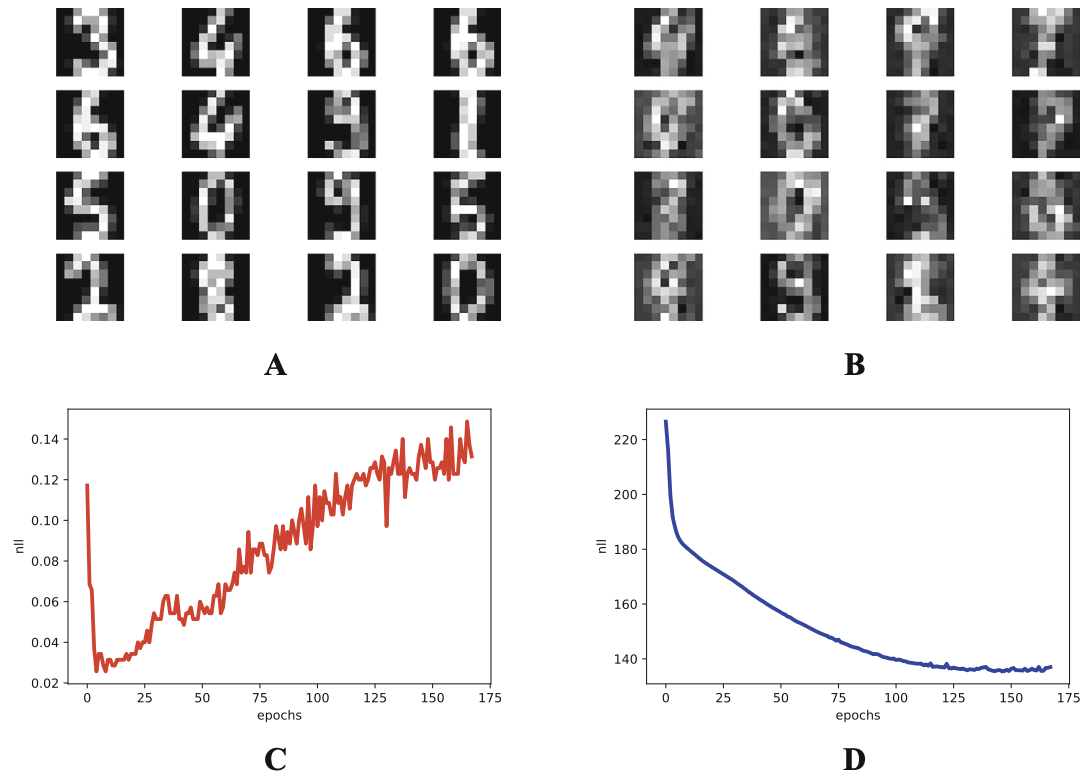
\includegraphics[width=\textwidth]{fig_6_4_hybrididf_outcomes.png}
\caption{Schematic summary of the HybridIDF training outcomes discussed in the
book's Fig.~6.4. The panels indicate the types of evidence shown there: real
validation images, unconditional samples, validation classification error, and
validation negative log-likelihood. This figure is an original conceptual redraw
for explanation and does not reproduce the original images or curves.}
\label{fig:hybrididf-outcomes}
\end{figure}

The first implication concerns out-of-distribution detection. The original
motivation for hybrid modeling was that \(p(y\mid x)\) alone cannot say whether
the input \(x\) is familiar. A density model \(p(x)\) can provide an additional
input-plausibility signal. In experiments by Nalisnick et al., hybrid models
with invertible features separated MNIST from NotMNIST and SVHN from CIFAR-10 in
likelihood-based evaluations~\cite{nalisnick2019hybrid}. These examples support
the idea that \(p(x)\) can help detect unfamiliar inputs. However, the conclusion
should remain modest. Likelihood is a useful signal, not a universal solution to
out-of-distribution detection. Its reliability depends on the data, the model
family, and the evaluation setting.

The second implication concerns semi-supervised learning. The hybrid objective
naturally separates labeled and unlabeled contributions. For labeled data, the
model can use the full objective \(\ell(x,y;\lambda)\). For unlabeled data, the
classification term is unavailable, but the density term \(\ln p(x)\) can still
be optimized. Because the backbone is shared, unlabeled data can improve the
representation used by the classifier. The book presents this point as one of
the natural directions for hybrid modeling~\cite{tomczak2024deep}. Nalisnick et
al. provide supporting evidence on MNIST, where adding unlabeled data improved
performance relative to using only a small labeled subset~\cite{nalisnick2019hybrid}.

This use case also clarifies why shared parameters are essential. Unlabeled data
can update the density term \(\ln p(x)\), and because the backbone is shared,
those updates can improve the representation used by the classifier. A separate
density model would not provide the same representation-level benefit.

The main limitation remains the weighting factor \(\lambda\). The parameter is
necessary because the predictive and generative terms operate on different
scales, but it also introduces a design choice that must be tuned. If
\(\lambda\) is too small, the density model may contribute little. If it is too
large, the representation may become biased toward density modeling at the
expense of classification. Moreover, when \(\lambda\neq 1\), the objective no
longer corresponds to the ordinary log of a normalized joint distribution. This
problem does not make the objective useless, but it does make the probabilistic
interpretation less clean.

The book's outlook points to several ways forward. Hybrid VAEs extend the same
idea beyond flows, but they require a variational lower bound instead of exact
likelihood evaluation. Other architectures or learning procedures may reduce the
need for a manually tuned \(\lambda\). The choice of factorization also remains
important. The factorization \(p(y\mid x)p(x)\) is well suited to reliable
decision-making because it keeps input plausibility explicit. A factorization
\(p(x\mid y)p(y)\) may be more natural when class-conditional generation is the
main goal. Finally, HybridIDF illustrates both the strength and the cost of
integer-valued flows: they match discrete data directly, but the rounding
operation requires the straight-through estimator and therefore biased
gradients.

\section{Conclusion}

Hybrid modeling reframes prediction as part of joint probabilistic modeling.
Instead of learning only \(p(y\mid x)\), the model also learns \(p(x)\). This
additional component gives the system a way to reason about input plausibility,
which is crucial when classifiers may encounter unfamiliar data. The central
factorization \(p(x,y)=p(y\mid x)p(x)\) therefore connects two goals: accurate
prediction and uncertainty-aware representation of the input space.

Normalizing flows make this connection practical because they provide invertible
features and exact likelihood evaluation. The same backbone can feed a
predictive head and support density modeling through the change of variables
formula. The derivation from naive separate models to shared parameterization
shows why this sharing matters: without shared parameters, the two terms can be
combined but do not learn together. With shared parameters, both the labels and
the input distribution shape the representation.

The weighted objective \(\ell(x,y;\lambda)\) is the technical hinge of the
framework. It compensates for the scale mismatch between a low-dimensional label
term and a high-dimensional input likelihood term. At the same time, it
introduces a hyperparameter and weakens the clean likelihood interpretation of
the objective. This trade-off is not a minor implementation detail; it is one of
the main conceptual tensions in hybrid modeling.

HybridIDF shows how the framework can be adapted to integer-valued data. By
using discrete bijections, the model avoids the continuous Jacobian term and
assigns probability mass directly to integer states. This construction fits
digital data more naturally than a continuous flow with dequantization. The price
is that integer-preserving transformations require rounding, and rounding
requires an approximate gradient estimator.

The broader lesson is that reliable decision-making benefits from both
predictive accuracy and a model of where the data distribution lies. Hybrid
models do not remove all difficulties of uncertainty estimation, but they make
the missing piece explicit. They ask a classifier not only to decide what an
input is, but also to model whether the input belongs to the world it has learned
to understand.

\bibliographystyle{splncs04}
\bibliography{references}

\end{document}
